\documentclass[11pt]{article}

\usepackage[a4paper,margin=25mm]{geometry}
\usepackage{amsmath,amssymb}
\usepackage{booktabs}
\usepackage{graphicx}
\usepackage{microtype}
\usepackage[numbers,sort&compress]{natbib}
\usepackage[hidelinks]{hyperref}

\graphicspath{{../figures/draft3/}}
\title{TopoDialogue III: Beyond the Transcript---Observable Implicit\\
Interactional Structure in Human--AI Dialogue}
\author{Ryoko Sakakibara\\Independent Researcher}
\date{16 August 2026}

\newcommand{\system}{\textsc{TopoDialogue}}
\newcommand{\code}[1]{\texttt{#1}}

\begin{document}
\maketitle

\begin{abstract}
What is often described as the ``unspoken'' part of human--AI dialogue should
not be operationalised by guessing a participant's hidden state. This paper
instead asks whether interactional structure that is not reducible to topic
content can be represented through observable, auditable events. We extend the
\system{} instrument with seven candidate event types: revisit, repair,
rejection, adoption, handover, reframing, and explicit pause. Each automatic
label is grounded in a visible surface marker, turn relation, or declared
lexical-recurrence rule; it is not treated as a gold annotation. We apply the
method to one 114-turn Japanese human--AI dialogue. Because automatic span
masking cannot establish anonymity, the public derivative withholds every
utterance and retains only speaker order, coarse descriptive metadata,
pseudonymous recurrence regions, and event candidates. The candidate extractor
finds 137 events, including 59 handovers, 33 reframings, 20 repairs, 14
rejections, 10 revisits, and one adoption. An event-enriched derivative changes
the operational revisit rate from 0.000 to 0.281 and LoopScore from 0.000 to
0.499 relative to the text-only fallback. This contrast is descriptive, not an
accuracy or causal result. Projection stability is only 0.207, demonstrating
that the displayed path is not robust enough to support interpretation by
shape alone. We provide deterministic extraction, a content-withheld release
format, an annotation guide, and per-label agreement software. Independent
human annotation has not yet been completed; agreement is therefore an explicit
gate for subsequent validation rather than a fabricated result.
\end{abstract}

\section{Introduction}

Dialogue contains more than propositions and topics. Speakers correct
themselves, refuse descriptions, accept proposals, return to earlier material,
and transfer the next move. These relations can matter even when the words do
not supply a stable thematic summary. Yet describing them as ``implicit'' can
invite an unsafe leap from an observed transcript to an unobserved intention,
emotion, or unconscious state.

This paper takes a narrower route. An implicit interactional structure is a
relation that is not represented by topic content alone but is observable in a
logged turn, a relation between turns, or an explicit interface event. Repair,
for example, has a long history as an interactional organisation rather than a
window into private mental content \citep{schegloff1977repair}. Dialogue-act
standards similarly show that communicative functions can be annotated through
declared schemes \citep{iso2020dialogue}. Mixed-initiative systems make the
allocation of control and initiative a design concern \citep{horvitz1999mixed}.
These traditions motivate labels whose evidence can be inspected and disputed.

\system{} began as a provenance-aware proposal for identifying recurrent,
low-progress regions and changing the co-ordinates of a dialogue rather than
asking indefinitely within one frame \citep{sakakibara2026concept}. Its second
paper fixed a reproducible trajectory instrument and distinguished closed
loops, spiral revisits, escapes, and open trajectories on synthetic cases
\citep{sakakibara2026instrument}. The present third paper asks what changes when
the instrument admits observable interaction events and a real conversation
without publishing its content.

The contributions are:
\begin{enumerate}
  \item an operational seven-label interaction-event protocol with explicit
        inclusion and exclusion rules;
  \item deterministic candidate extraction with evidence provenance and a
        distinction between automatic candidates and human gold labels;
  \item a content-withheld derivative that reproduces released aggregate
        analyses without releasing utterances;
  \item a pilot application to a 114-turn Japanese human--AI dialogue; and
  \item agreement software and a declared two-annotator validation gate,
        including undefined handling for labels absent from both files.
\end{enumerate}

We do not claim to recover unspoken thoughts, infer affect, diagnose a person,
establish a mathematical topological invariant, or show that the event-enriched
representation is better. The study is an instrumentation pilot.

\section{Related positioning}

Computational work on dialogue dynamics motivates analysing movement and
interactional development alongside content \citep{fischer2024trajectories}.
Summaries of interactional dynamics have also been evaluated separately from
the facts and opinions expressed in a transcript \citep{hua2024dynamics}.
However, a trajectory picture remains a measurement display rather than an
explanation. The earlier \system{} instrument made this distinction explicit
through input hashes, projection seeds, operational recurrence, and artefact
warnings \citep{sakakibara2026instrument}. The present work preserves that
boundary and adds events that can be checked against a transcript.

The event inventory is deliberately smaller than a general dialogue-act
taxonomy. ISO 24617-2 provides a multidimensional framework for dialogue-act
annotation \citep{iso2020dialogue}; our labels instead target recurrence and
change within a single trajectory. Repair is grounded in overt correction or
reformulation, consistent with conversation-analytic attention to the
organisation of repair \citep{schegloff1977repair}. Handover is a structural
candidate when question punctuation is followed by a speaker change. It is not
a claim that the speaker intended to relinquish control. Adoption and rejection
refer to explicit uptake or refusal of a proposal or frame, while reframing
requires an overt substitution of viewpoint, assumption, or abstraction.

Inter-coder agreement is not a decorative reliability number. Different
coefficients answer different questions, prevalence affects chance-corrected
statistics, and degenerate categories require careful handling
\citep{artstein2008agreement}. We therefore report no human agreement in this
pilot. The software emits Cohen's kappa, observed agreement, and positive-class
F1 per label only after two independently produced files are supplied.

\section{Method}

\subsection{Observable event schema}

Let the normalised dialogue be $D=(u_1,\ldots,u_T)$. An event is
$e=(i,\ell,b,c,a)$, where $i$ identifies a turn, $\ell$ is one of seven labels,
$b$ records the evidence basis, $c\in[0,1]$ is extractor confidence, and $a$ is
an optional earlier anchor turn. The bases are \emph{surface marker},
\emph{turn structure}, and \emph{lexical recurrence}. Confidence indicates rule
specificity; it is not an empirical probability of correctness.

\begin{table}[t]
\centering
\small
\caption{Operational event inventory.}
\label{tab:events}
\begin{tabular}{p{21mm}p{94mm}}
\toprule
Label & Observable condition \\
\midrule
revisit & Character-trigram Jaccard similarity of at least 0.10 to a non-adjacent earlier turn. \\
repair & Explicit correction or reformulation marker, such as ``more precisely'' or Japanese equivalents. \\
rejection & Explicit refusal of a proposal or description; ordinary explanatory negation is excluded. \\
adoption & Explicit acceptance of a proposal or frame for subsequent use. \\
handover & Question punctuation followed by a change of speaker. \\
reframing & Explicit substitution of viewpoint, premise, constraint, or abstraction. \\
pause & An explicit pause, silence, interruption, or resume marker in the log. \\
\bottomrule
\end{tabular}
\end{table}

The threshold 0.10 is fixed for this pilot after inspecting the behaviour of
long Japanese turns; it is not claimed to generalise. Immediate neighbours are
excluded from recurrence. Ellipses and fillers do not produce pause labels.
Japanese explanatory negation is not itself rejection. A turn may receive
multiple labels because, for example, a repair may also introduce a reframing.

The surface-marker inventory is Japanese-specific in this pilot. It is not a
universal codebook that can be transferred unchanged across languages,
communities, relationships, or tasks. A new setting requires a versioned marker
pack, independently annotated examples, and threshold evaluation on held-out
dialogues. Event frequencies must not be used to infer a participant's culture,
nationality, personality, or preferred degree of directness.

\subsection{Privacy-preserving real-case preparation}

The source case was selected from the author's own archived human--AI
conversations because it had balanced speakers (57 user and 57 assistant turns)
and did not concern sleep, finance, health, or account administration. The raw
dialogue contains 69,030 characters and remains local. A pattern audit found
two URLs and 11 date-or-time-like strings, but absence of such patterns would
not establish anonymity. Context can identify a person without matching a
regular expression.

Consequently, the released object does not perform selective redaction. Every
utterance becomes a placeholder such as \code{[content withheld; medium turn]}.
The derivative retains speaker order, turn index, a coarse length bin,
question/statement form, pseudonymous region identifiers, and event candidates.
Evidence hashes and character offsets are removed. Only pseudonymous region and
event keys enter the released trajectory. Length and form remain metadata;
including those common bins as trajectory features created artificial revisits
during development and was rejected.

The raw case has a SHA-256 fingerprint so the author can verify local source
identity. The fingerprint does not make the source public and should not be
interpreted as anonymous proof. A scan over 116 source strings of at least 20
characters found no exact occurrence in the public derivative.

\subsection{Trajectory comparison}

The text-only fallback and public event derivative are processed by the same
\code{trajectory-v1} analyser. For feature sets $F_t$ and $F_j$, recurrence uses
Jaccard similarity
\begin{equation}
s(t,j)=\frac{|F_t\cap F_j|}{|F_t\cup F_j|}.
\end{equation}
The trajectory analyser declares a revisit at $s\geq0.5$, separately from the
0.10 candidate threshold used to create pseudonymous raw-text regions.
LoopScore is the mean revisit similarity multiplied by one minus mean
operational progress, clipped to $[0,1]$. These are software quantities, not
calibrated measures of quality or psychological state.

The comparison is not a controlled ablation: the public derivative intentionally
removes words and adds event keys. It demonstrates representational sensitivity
and reproducibility, not superiority. Projection stability is the correlation
of pairwise distances under two deterministic projection seeds. A low value is
an artefact warning, not a negative judgement about the conversation.

\subsection{Independent annotation gate}

Two annotators must label the same turn identifiers independently using the
published inclusion and exclusion rules. The comparison programme requires
identical turn universes and produces per-label observed agreement, Cohen's
kappa, and positive-class F1. If both annotators assign no instances of a
label, kappa and F1 are recorded as undefined rather than perfect. Automatic
candidates are compared with adjudicated labels only after the independent
report is frozen. This study implements and tests that process but does not
claim it has been performed by two people.

\section{Results}

\subsection{Candidate events in the real case}

The deterministic extractor produced 137 candidates across 114 turns
(Table~\ref{tab:counts}; Figure~\ref{fig:counts}). No explicit pause marker was
present. Handover is frequent because many questions are followed by a speaker
change. This should not be read as 59 intentional transfers of control.

\begin{table}[t]
\centering
\caption{Automatic surface/structure candidates in the real case.}
\label{tab:counts}
\begin{tabular}{lr@{\qquad}lr}
\toprule
Event & Count & Event & Count \\
\midrule
handover & 59 & reframing & 33 \\
repair & 20 & rejection & 14 \\
revisit & 10 & adoption & 1 \\
pause & 0 & total & 137 \\
\bottomrule
\end{tabular}
\end{table}

\begin{figure}[t]
\centering
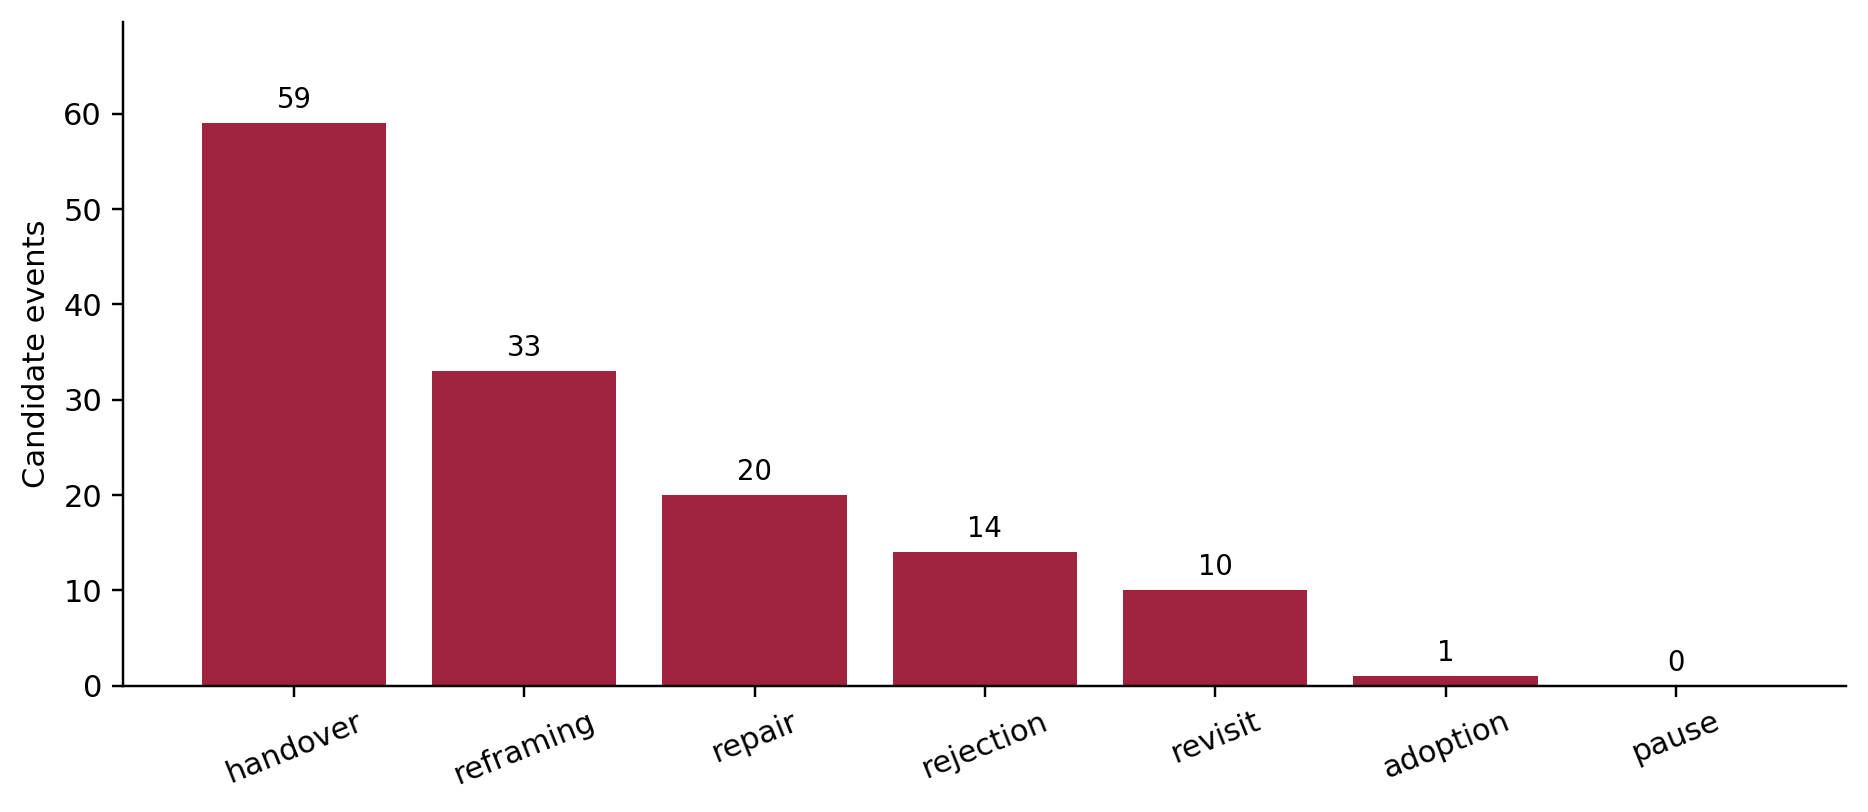
\includegraphics[width=\linewidth]{event-counts.png}
\caption{Candidate counts. The bars show deterministic extractor output, not
human-validated frequencies.}
\label{fig:counts}
\end{figure}

\subsection{Representation-sensitive trajectory}

Table~\ref{tab:comparison} and Figure~\ref{fig:comparison} show the diagnostic
contrast. The lexical fallback detects no operational revisit at the analyser's
0.5 threshold. The public event derivative detects 32, with revisit rate 0.281,
mean revisit similarity 0.601, and LoopScore 0.499. Escape@5 is true under the
finite software rule. These changes show that interaction-event coding changes
the state representation. They do not show that 32 is the correct natural-language
count, that an ``escape'' occurred for the person, or that the event representation
is more accurate.

\begin{table}[t]
\centering
\small
\caption{Descriptive comparison on one case.}
\label{tab:comparison}
\begin{tabular}{lrr}
\toprule
Metric & Text fallback & Event derivative \\
\midrule
Turns & 114 & 114 \\
Operational revisits & 0 & 32 \\
Revisit rate & 0.000 & 0.281 \\
Mean revisit similarity & 0.000 & 0.601 \\
LoopScore & 0.000 & 0.499 \\
Escape@5 & No & Yes \\
Projection stability & 0.479 & 0.207 \\
\bottomrule
\end{tabular}
\end{table}

\begin{figure}[t]
\centering
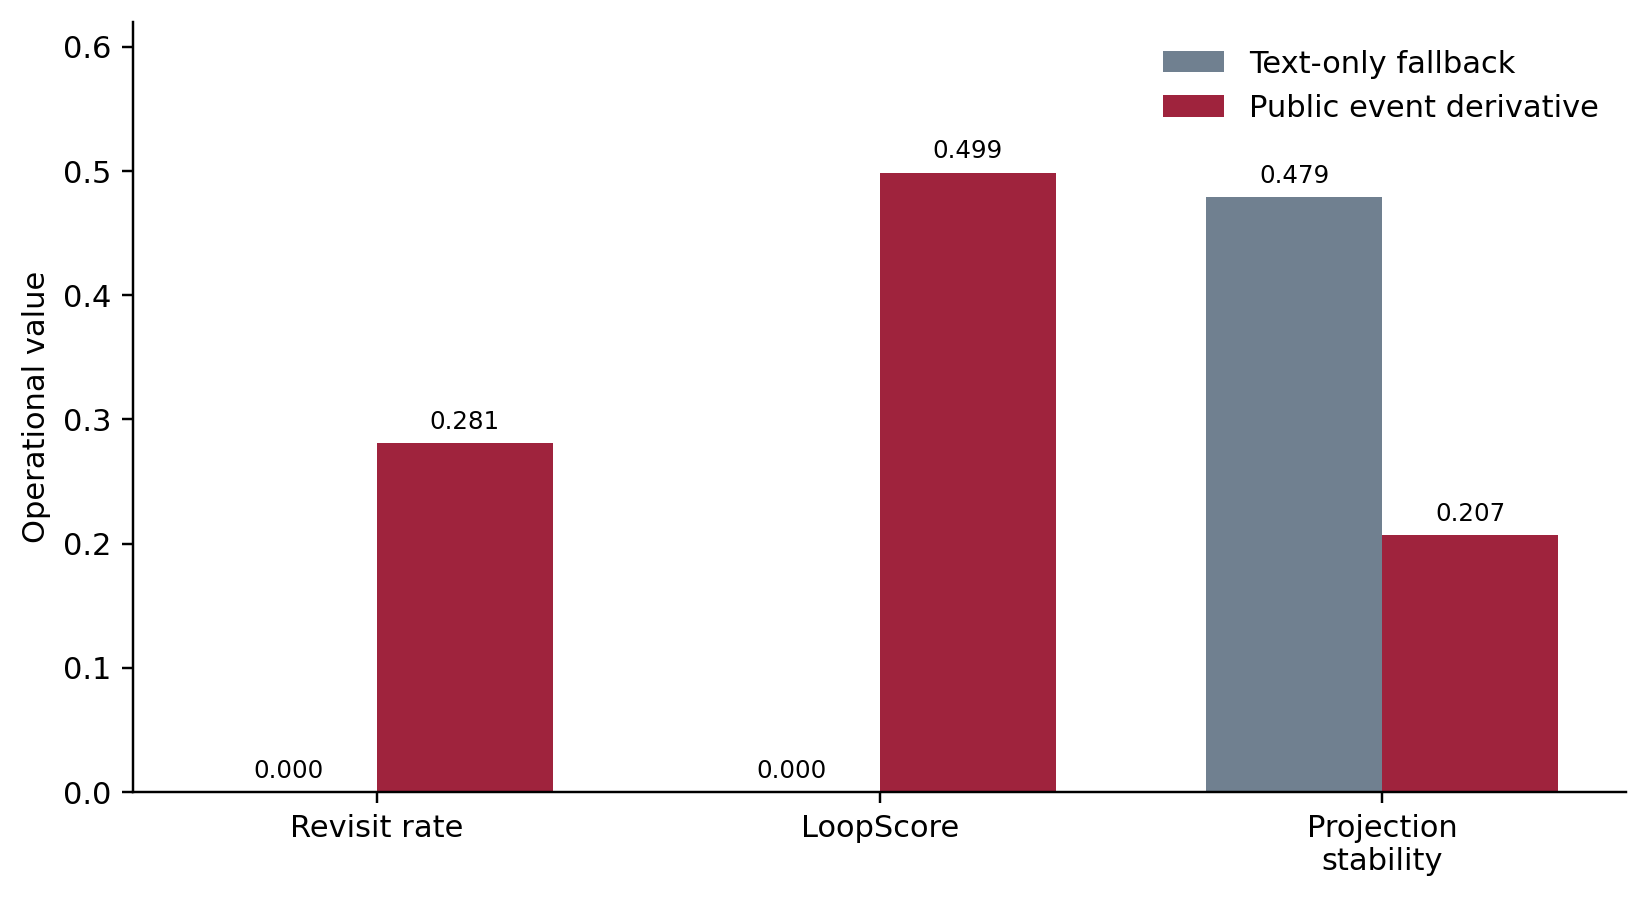
\includegraphics[width=\linewidth]{baseline-comparison.png}
\caption{Representation-sensitive operational values. This is not an accuracy
comparison because the feature contracts differ by design.}
\label{fig:comparison}
\end{figure}

The two-dimensional display in Figure~\ref{fig:trajectory} is deliberately
included with its failure signal. The event derivative forms clusters and long
crossing segments, but projection stability is 0.207, below the instrument's
0.65 warning threshold. A different deterministic projection can materially
change the silhouette. The circled points are operational revisits under the
feature rule; they are not inferred returns to an inner mental state.

\begin{figure*}[t]
\centering
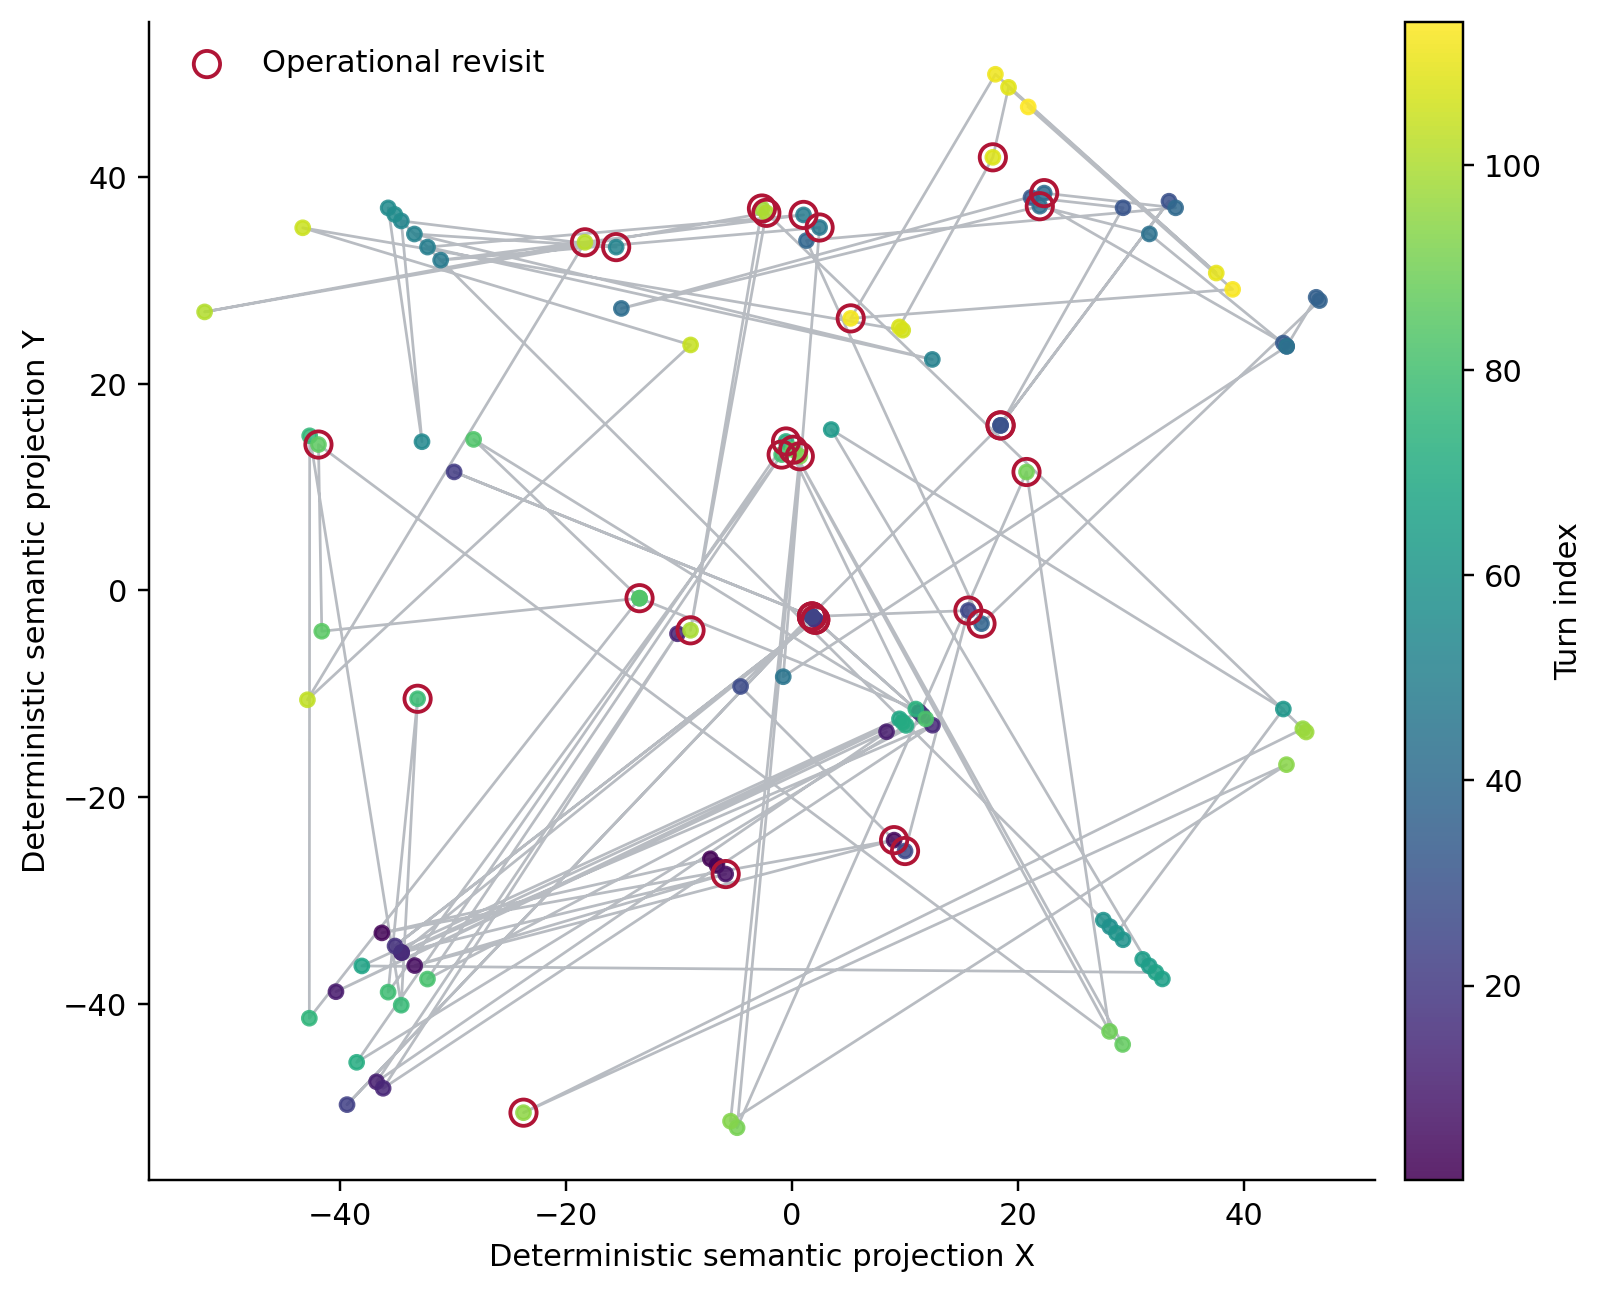
\includegraphics[width=0.82\textwidth]{public-trajectory.png}
\caption{Content-withheld event trajectory. Colour encodes turn order and red
rings mark operational revisits. Low projection stability prevents
interpretation of the particular planar silhouette.}
\label{fig:trajectory}
\end{figure*}

\subsection{Reproducibility checks}

The Python suite contains 19 passing tests, including deterministic extraction,
privacy withholding, rejection false-positive regression, agreement edge cases,
and trajectory reproduction. Eight JavaScript tests cover the browser
trajectory analysis, including preservation of public event features. The raw
input is not needed to regenerate the released figures: the event-count and
trajectory figures consume the public JSON and aggregate report. Repeated runs
retain the same event sequence, feature keys, input hash, and metrics.

\section{Failure cases and threats to validity}

\paragraph{Marker ambiguity.}
``Another perspective'' can describe content without performing a reframe.
Question punctuation can be rhetorical. Explicit acceptance can be quoted
rather than adopted. Rule confidence is therefore not annotation accuracy.

\paragraph{Japanese segmentation.}
Character trigrams avoid requiring a segmenter but are sensitive to orthography,
formulaic phrasing, and turn length. The 0.10 pilot threshold was not estimated
on an independent corpus. A lexical revisit count of zero at the stricter
trajectory threshold illustrates this mismatch.

\paragraph{Cultural and relational transportability.}
The same surface form may perform different interactional work across
languages, communities, relationships, status configurations, and tasks.
Conversely, the same interactional work may be realised by different forms.
Even a familiar national-level generalisation---that Japanese speakers are
more indirect than American speakers---was not supported across the matched
request and complaint situations examined by Spees \citep{spees1994indirectness}.
The present single Japanese case cannot separate language, culture, dyad,
individual history, or task. Cross-setting use therefore requires comparison
against three declared references: the participant's own prior distribution,
the distribution of the particular human--AI relationship, and the current
task context. These are calibration strata, not demographic profiles.

\paragraph{Missing interface events.}
The export contains final turns, not editing, regeneration, copying, dwell time,
or abandoned drafts. An absent pause event means no explicit marker was logged;
it does not mean that no pause occurred.
The source is a text export: source audio and prosody, sign, gaze, symbol,
switch, tactile, and augmentative interactions were not observed. Equivalent
text therefore does not establish an equivalent interactional event across
interfaces. Measuring such conversion loss is reserved for Paper IV.

\paragraph{Privacy and verifiability.}
Withholding all text reduces disclosure but prevents a public reader from
auditing the semantic appropriateness of each candidate. The raw fingerprint
supports local identity checking, not external verification. Controlled access
or independently consented corpora are needed for stronger replication.

\paragraph{Single-case design.}
The event frequencies and metric changes describe one conversation selected by
its author. They do not generalise to other people, models, languages, or tasks.
No performance, behavioural, or causal claim follows.

\paragraph{No human agreement yet.}
Software conformance is not annotation reliability. The two-annotator gate is
unmet. Until it is completed, the label counts remain candidates and the paper
should be read as a protocol plus pilot, not a validated coding study.

\section{Discussion}

The pilot clarifies what ``beyond the transcript'' can responsibly mean. It
does not mean beneath consciousness or outside language. It means beyond a
bag of topical content: the observable organisation of correction, uptake,
refusal, return, and control of the next move. This definition turns a broad
philosophical intuition into disputable records.

The strongest result is methodological rather than numerical. Common metadata
features initially generated many false revisits. Removing length and
question/statement bins from the trajectory while retaining them as descriptive
metadata materially reduced that artefact. The low projection stability of the
remaining real-case path supplies a second warning: a visually compelling
curve cannot substitute for a stable operational report.

The next empirical step is bounded. Two independent annotators should label a
small, consented set, freeze the agreement report, adjudicate disagreements,
and compare automatic candidates with adjudicated labels. Thresholds should
then be evaluated on held-out conversations. Only after that evidence should
the project add learned event models, interface telemetry, multimodal signals,
persistent homology, or other topological data analysis.

This transportability boundary also fixes the next two papers' roles. Paper IV
should test whether individual, relationship, and context baselines improve
event calibration before adding optional embodied or interface signals. Paper V
should then evaluate adaptive interaction strategies: which question,
reframing, wait, or return is helpful in a particular context, as evidenced by
subsequent adoption, rejection, repair, and user correction. This is not a
claim to infer a stable personality. Retrieval-augmented generation may supply
past episodes and a graph may store their relations, but neither by itself
defines the adaptation policy or its user-controlled evaluation.

\section{Conclusion}

\system{} III represents implicit interactional structure without claiming
access to hidden mental content. It provides seven observable event candidates,
provenance, a content-withheld real-case derivative, deterministic figures, and
agreement tooling. On one 114-turn Japanese dialogue, event coding changes the
operational recurrence report, while low projection stability prevents shape
interpretation. The result is a reproducible pilot and a concrete human-validation
gate. It is not a psychological reading of the participant and not evidence
that a particular geometric silhouette is true. Its marker inventory is a
language-specific starting point, not a culturally universal model.

\section*{Data and software availability}

The release bundle contains the English manuscript, Japanese companion, source,
figures, event protocol, and content-withheld derivative. The raw conversation
is not released. The first two \system{} papers are archived at
\url{https://doi.org/10.5281/zenodo.21962837} and
\url{https://doi.org/10.5281/zenodo.21963131}.

\section*{Ethics statement}

The pilot uses an author-controlled conversation and releases no utterance
content. Event candidates are not mental-state, clinical, or diagnostic labels.
No other human annotator participated in the reported results. A future study
with additional annotators or participants requires consent, role disclosure,
and an appropriate data-access plan.

\bibliographystyle{plainnat}
\bibliography{references}
\end{document}
